\fxnote{Add interactive somewhere in the research question}
\fxnote{Who is the target audience?}
\chapter{Creating an interactive map}
When creating an interactive map one must consider which features to add to enhance the user experience. To give an overview of some of the basic features used for navigating and get information from a map an example of an interactive map has been used. www.openstreetmap.org has been used as an example of an interactive map. A picture of this map can be seen in figure x. Its User Interface (UI) have been numbered with boxes, which have been colored green if the feature would make sense for exploring and comparing large population dataset.  
www.openstreetmap.org

\begin{figure} [H]
	\centering
	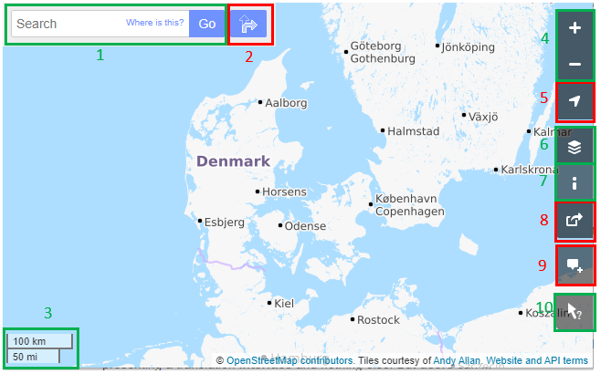
\includegraphics[width=.8\textwidth]{Pictures/InteractiveMap}
	\caption{An example of an interactive map}
	\label{InteractiveMap}
\end{figure}

\begin{table}[htbp]
	\centering
	\begin{tabular}{l}
		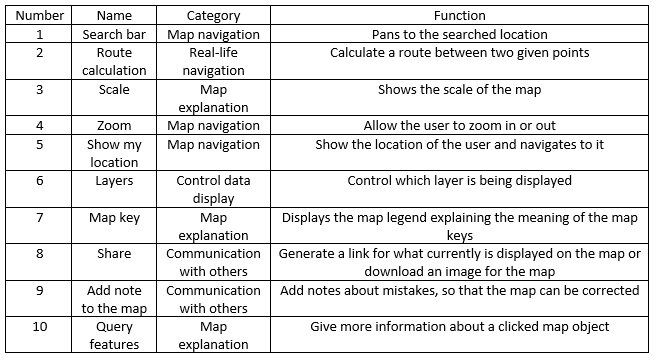
\includegraphics[width=0.8\textwidth]{Pictures/tabOSMFunctions}
	\end{tabular}
	\caption{Overview of the UI elements highlighted in figure \ref{InteractiveMap}}
	\label{tabOSMFunctions}
\end{table}

What the different parts of the UI does can be seen in table x. The functions of the UI can be classified in five different categories. Using the map navigation UI the user can control which part of the map is being displayed.
The real-life navigation tool is used for navigating in the real world. 
The map explanation category gives the user information about the map. This can be general information about the scale or symbols on the map or specific information about a clicked point. 
The tool for controlling the displayed data is used for controlling what is being visualized on the map.
The last category, communication with others, is for sharing information with other users of the map. 
\fxnote{Write that my own search bar can be improved} 
\fxnote{Did I write about toogling dual legends?} 
